\documentclass[onecolumn, draftclsnofoot, 10pt, compsoc]{IEEEtran}
\usepackage{graphicx}
\usepackage{url}
\usepackage{setspace}
\usepackage{geometry}

\geometry{textheight=9.5in, textwidth=7in}

% @here - we should consider modifying this, it looks kind of weird and lacks some of the info I'd like to have + this year's logo
% 1. Fill in these details
\def \CapstoneTeamName{			Team 12}
\def \CapstoneTeamNumber{		12}
\def \GroupName{				CS Capstone Team }
\def \GroupMemberOne{			Trey Elkins}
\def \GroupMemberTwo{			Leif Tsang}
\def \GroupMemberThree{			Ryan Wallerius}
\def \CapstoneProjectName{		NASA USLI Rocket Team}
\def \CapstoneSponsorCompany{	Oregon State University}
\def \CapstoneSponsorPerson{	Dr. Nancy Squires}

% 2. Uncomment the appropriate line below so that the document type works
\def \DocType{		%Problem Statement
					Requirements Document
					%Technology Review
					%Design Document
					%Progress Report
				}
			
\newcommand{\NameSigPair}[1]{
	\par
	\makebox[2.75in][r]{#1} \hfill
	\makebox[3.25in]{\makebox[2.25in]{\hrulefill} \hfill \makebox[.75in]{\hrulefill}}
	\par\vspace{-12pt}
	\textit{
		\tiny\noindent \makebox[2.75in]{} \hfill
		\makebox[3.25in]{\makebox[2.25in][r]{Signature} \hfill \makebox[.75in][r]{Date}}
	}
}
% 3. If the document is not to be signed, uncomment the RENEWcommand below
\renewcommand{\NameSigPair}[1]{#1}
\renewcommand{\thesubsubsection}{\thesection.\alph{subsubsection}}

%%%%%%%%%%%%%%%%%%%%%%%%%%%%%%%%%%%%%%%
\begin{document}
\begin{titlepage}
    \pagenumbering{gobble}
    \begin{singlespace}
    	%\includegraphics[height=4cm]{coe_v_spot1}
        \hfill 
        % 4. If you have a logo, use this includegraphics command to put it on the coversheet.
        %\includegraphics[height=4cm]{CompanyLogo}
        \begin{center}
           
\includegraphics[scale = 0.2]{2019patch.png}\\[1.0 cm]

        \par\vspace{.2in}
        \scshape{
            \huge CS Capstone \DocType \par
            {\large\today}\par
            \vspace{.5in}
            \textbf{\Huge\CapstoneProjectName}\par
            \vfill
            {\large Prepared for}\par
            %\Huge \CapstoneSponsorCompany\par
            \vspace{5pt}
            {\Large\NameSigPair{\CapstoneSponsorPerson}\par}
            {\large Prepared by }\par
           	\GroupName\par
            % 5. comment out the line below this one if you do not wish to name your team
            %\CapstoneTeamName\par
            \vspace{5pt}
            {\Large
                \NameSigPair{\GroupMemberOne}\par
                \NameSigPair{\GroupMemberTwo}\par
                \NameSigPair{\GroupMemberThree}\par
            }
            \vspace{20pt}
        }
        \end{center}
    \end{singlespace}
    
    \begin{abstract}
    	% 6. Fill in your abstract
        This document outlines the client requirements for the computer science portion of the Oregon State University's entry into the NASA University Student Launch Initiative. The systems outlined in this requirements document entail rocket tracking and avionics, rover payload operations, and management of the team website.
	\end{abstract}
\end{titlepage}
\newpage

\pagenumbering{arabic}
\tableofcontents
% 7. uncomment this (if applicable). Consider adding a page break.
%\listoffigures
%\listoftables
\clearpage

\section{Revision Table}
Sections have been incremented by 1 from our drafts to our final draft because of the addition of the revision table. 
\begin{table}[h]
\centering
\begin{tabular}{|l|l|l|}
\hline
Section & Original & New \\ \hline
1.3,1.6 & Overview & \begin{tabular}[c]{@{}l@{}}Now merged into 2.3 'Scope'. Some portions\\ also removed/rewritten\end{tabular} \\ \hline
2.4 & Definitions & Added some definitions \\ \hline
2.1.1-2.1.3 now 3.2 & System Interfaces & All rewritten and rephrased \\ \hline
3.2 & N/A & Added Rover Section \\ \hline
3.3.3 & N/A & Added Website functions: \\ \hline
3.1 & N/A & Added gps to overall description. \\ \hline
3.1 & N/A & Made payload operation more general \\ \hline
4 & System features & \begin{tabular}[c]{@{}l@{}}All written and expanded upon, final requirements\\ outlined and clarified\end{tabular} \\ \hline
\end{tabular}
\end{table}

\section{Project Overview}
\subsection{Introduction}
The NASA Student Launch is a competitive experiential exploration and learning activity. It strives to provide relevant, cost-effective, grassroots research and development in the field of rocket propulsion and launch systems. This project offers multiple challenges reaching a broad audience of middle and high schools, colleges, and universities across the United States.

\subsection{Purpose}
This document outlines the customer and competition requirements for the Computer Science team participating in Oregon State University's entry into the 2019 NASA Student Launch Initiative. 

\subsection{Scope} %Ryan will update the content in this section 
This document contains the complete software requirements and specifications for the computer science portion of the NASA University Student Launch Initiative.  The software can be organized into three parts:

\begin{enumerate}
\item \textbf{Launch Vehicle Avionics and Telemetry}, active tracking, logging, filtering, and transmission of coordinate data to a ground station.
\item \textbf{Payload Software}, must maneuver 10 feet away from the landed rocket with object avoidance and collect a soil sample specified by the competition requirements.
\item \textbf{Website}, the location where NASA will receive design and technical documents required for the competition as well as a place to display other information and facts about the team.
\end{enumerate}

This document has been updated to reflect changes in customer requirements specified by NASA personnel and the team administration over the course of the competition.

% @here - this sucks, let's fix it?
\subsection{Definitions, acronyms, and abbreviations}
\begin{center}
  \begin{tabular}{|l|l|}
      \hline
      AIAA	&American Institute of Aeronautics and Astronautics\\
      \hline
      CS		&Computer Science\\
      \hline
      ECE		&Electrical and Computer Engineering\\
      \hline
      ME		&Mechanical Engineering\\
      \hline
      OSU		&Oregon State University\\
      \hline
      USLI		&University Student Launch Initiative\\
      \hline
      GPS       &Global Positioning System\\
  \end{tabular}
\end{center}

% @here - we need to make sure formatting is consistent with IEEE standard and/or what we've been doing for our other assignments, ex. add \noindent if necessary

\section{Overall description}
\subsection{Product Perspective}
The launch vehicle avionics system will collect and log coordinate data from on-board GPS sensors. Data will be used for analysis of launch vehicle flight profile and drift radius for reporting in NASA documentation, as well as for recovery of the launch vehicle after flight.

The rover payload will use sensors to complete the rover mission along with GPS in order to move at least the specified distance away from the launch vehicle. The program will be written and managed by the CS team. The CS team will be in contact with the ECE team on decisions made for payload management and operations. 

The Website will not be graded in the competition itself but is crucial for storage and retrieval of key technical documentation required by NASA for competition purposes. The Website will be managed and created by the CS team and will be published on a domain purchased by the OSU USLI Team. 

\subsection{System interfaces}
The launch vehicle avionics software will interact with the GPS sensors and data logging via a Teensy 3.6 microcontroller running Arduino code. 
\vspace{.5cm}

\noindent The rocket avionics will interact with GPS sensors on-board the rocket to collect coordinate data during the flight via a serial interface. The Teensy will manage an XBee Pro S3 900 MHz transceiver (also via serial) that packs filtered data and sends it to a ground station utilizing similar hardware for data output and recovery purposes. The flight units are equipped with SD cards that log the data to text files for later recovery and analysis.
\vspace{.5cm}

\noindent The payload software will control the rover through both a Teensy 3.6 microcontroller and BeagleBone Black microcomputer. The Teensy will run the primary script while the BeagleBone will be continuously processing images through computer vision. The BeagleBone will be connected to the Teensy via UART sending the Teensy instructions based off of processed images. All sensors and components will be directly connected to the Teensy. The Teensy will pull information from these sensors as necessary for the payload mission. 
\vspace{.5cm}

\noindent The Website will be hosted on a domain purchased by the OSU USLI team via the Github.io web service.


% @here - website??

\subsection{Product Functions}
\subsubsection{Avionics Functions} \begin{itemize}
\item Read coordinate data from GPS sensors.
\item Log and filter GPS data.
\item During flight, avionics will transmit data to ground station. 
\item Ground station displays serial data to host PC.
\item After flight, ground station transmits trigger signal to payload ejection controller.\\
\end{itemize}

% @here - consistent formatting, also lets update this
\subsubsection{Payload Functions} \begin{itemize}
\item Read data from individual sensors.
\item Be able to properly use object avoidance. 
\item Drive at least ten feet away from the landed rocket and collect a soil sample. \\
\end{itemize}

\subsubsection{Website Functions} \begin{itemize}
\item Host critical NASA documents. 
\item Enable downloading of documents.
\item Present information on the team and project.
\end{itemize}

\subsection{User Characteristics}
The intended users of these systems will be primarily ECE and CS team members - typically college-aged students familiar with software and high level electronics. The primary exception to this is the website, which will need to be navigable and easily usable by any adult, though the real target users will be NASA engineers, members of other teams, and potential sponsors who are curious about our team and documentation.

\subsection{Constraints}
\subsubsection{Regulatory Policies}
Competition restrictions dictate that our approach to various problems must accommodate competition requirements. Everything must comply with federal law and with the requirements enumerated in the Student Launch Initiative handbook. Exceptions or changes are at the discretion of the NASA committee orchestrating the competition. We cannot, for instance, transmit flight guidance data to the rocket as that would legally classify it as a guided missile. Another instance of competition policy is the requirement that all transceivers operate under 250 mW of power draw to minimize interference.

\subsubsection{Memory and Processing Constraints}
Both avionics and payload software must comply with the memory and processing constraints of the Teensy 3.6 as well as buffer and serial constraints of the XBee Pro S3 transceiver. Serial monitors and scripts can be run on Windows machines or any other computer that has support for standard programming languages.

\subsubsection{Interfaces to Other Applications}
Outside of situations such as radio-frequency interference, our systems must not interrupt or compromise the operation of any other team's systems at competition. In cases where all interaction cannot be eliminated - such as in use of commonplace radio-frequency bands - measures must be taken to minimize impact on the systems of other teams.

\subsubsection{Higher-Order Language Requirements}
Both the avionics and rover payload software must be written in a high level programming language such as the Arduino programming language. The website must also be implemented using tools or libraries other than just basic HTML, CSS, and JavaScript.

% @here - this is BS
\subsubsection{Safety and Security Considerations}
The rocket will launch far enough away from spectators not to pose a safety threat. All bystanders must be far enough away from the PLEC receiver that the black powder charges and payload ejection don't cause any personal bodily harm.

% @here - lol nah
\subsection{Assumptions and Dependencies}
The ECE/ME team will provide the computer hardware necessary to run the Rocket and Payload Programs. The ECE team will provide the CS team with sufficient time and information to test and debug our software using their final version of the flight hardware. Development will be supported by an array of standard libraries, with some non-standard libraries being used where possible and applicable. The team will be operating with a minimal budget - almost all hardware should be provided by AIAA or the USLI team, but some budgetary contributions might be necessary to secure the correct materials, especially if said materials aren't readily available through the CS capstone program.

% @here - this needs heavy revisiting (Just trey's lul)
\section{Specific Requirements}
\subsection{System Features}
\subsubsection{Avionics} \begin{enumerate}
\item \textbf{Code Refactor:} Code must be streamlined and documented, with at least a 25\% reduction in lines of code and thorough commenting. 
\item \textbf{Broadcasting:} Avionics system must be capable of receiving GPS data and transmitting to the ground station with enough fidelity that the rocket can be recovered using the data after flight.
\item \textbf{Output:} Ground station must print to serial monitor on host PC so that data can be viewed and retrieved remotely.
\item \textbf{Data Logging and Storage:} Flight data must be logged, stored, and easily recoverable for data analysis.
\item \textbf{Ejection Control:} The ground station must be capable of sending an ejection signal to the payload ejection controller (PLEC) that will trigger black powder charges and eject the rover.
\item \textbf{433 MHz Prototype:} The 433 MHz prototype must be capable of transmission of plaintext data wirelessly between two separate units.
\end{enumerate}
\subsubsection{Payload Software}


\begin{enumerate}
\item \textbf{Traversal away from air frame} The rover must move at least ten feet away from the landed rocket using a GPS distance algorithm
\item \textbf{Movement} The rover will have robust slow start and slow halt and turn movement features
\item \textbf{Object avoidance} The rover must avoid any large objects utilizing 2 front mounted sonar 
\item \textbf{Soil Collection} The rover must drill for a soil sample utilizing an on board auger with a sealed collection chamber
\item \textbf{GPS} The rover will use GPS in order to record locations of collected soil and transmit the location to a ground station
\item \textbf{Magnetometer} The magnetometer will be able to output an integer ranging from 0 - 359 based on the heading of the rover
\item \textbf{Gyroscope} The rover will be able to use the Gyro in order to detect levelness of the rover at any given time
\item \textbf{Routing Algorithms} Routing algorithms will be in place to allow the rover to navigate based on GPS coordinates
\item \textbf{Logging} The rover will have the ability to log information to a microSD card on the teensy
\item \textbf{Computer Vision} The Beaglebone black on board the rover will be able to capture images and process each image for a target which will have the location transmitted via UART to the Teensy. 
\end{enumerate}


\subsubsection{Website}
The website will have the following features: 
\begin{itemize}
    \item \textbf{Home Page:} The home page will have the OSU USLI team's mission statement and mission picture. 
    \item \textbf{About Us:} The about us page will have a list of the capstone seniors that are working on the page. This will include names, email addresses, the program they are in, and the system they are working on. 
    \item \textbf{Deliverables:} The deliverables page will have all of the critical NASA documents needed for competition. Anyone will be able to access this page and download any document on the page. 
\end{itemize}
All of this will be done using ReactJS framework. 

\subsection{Development Chart Timeline}
\begin{center}
  \makebox[\textwidth]{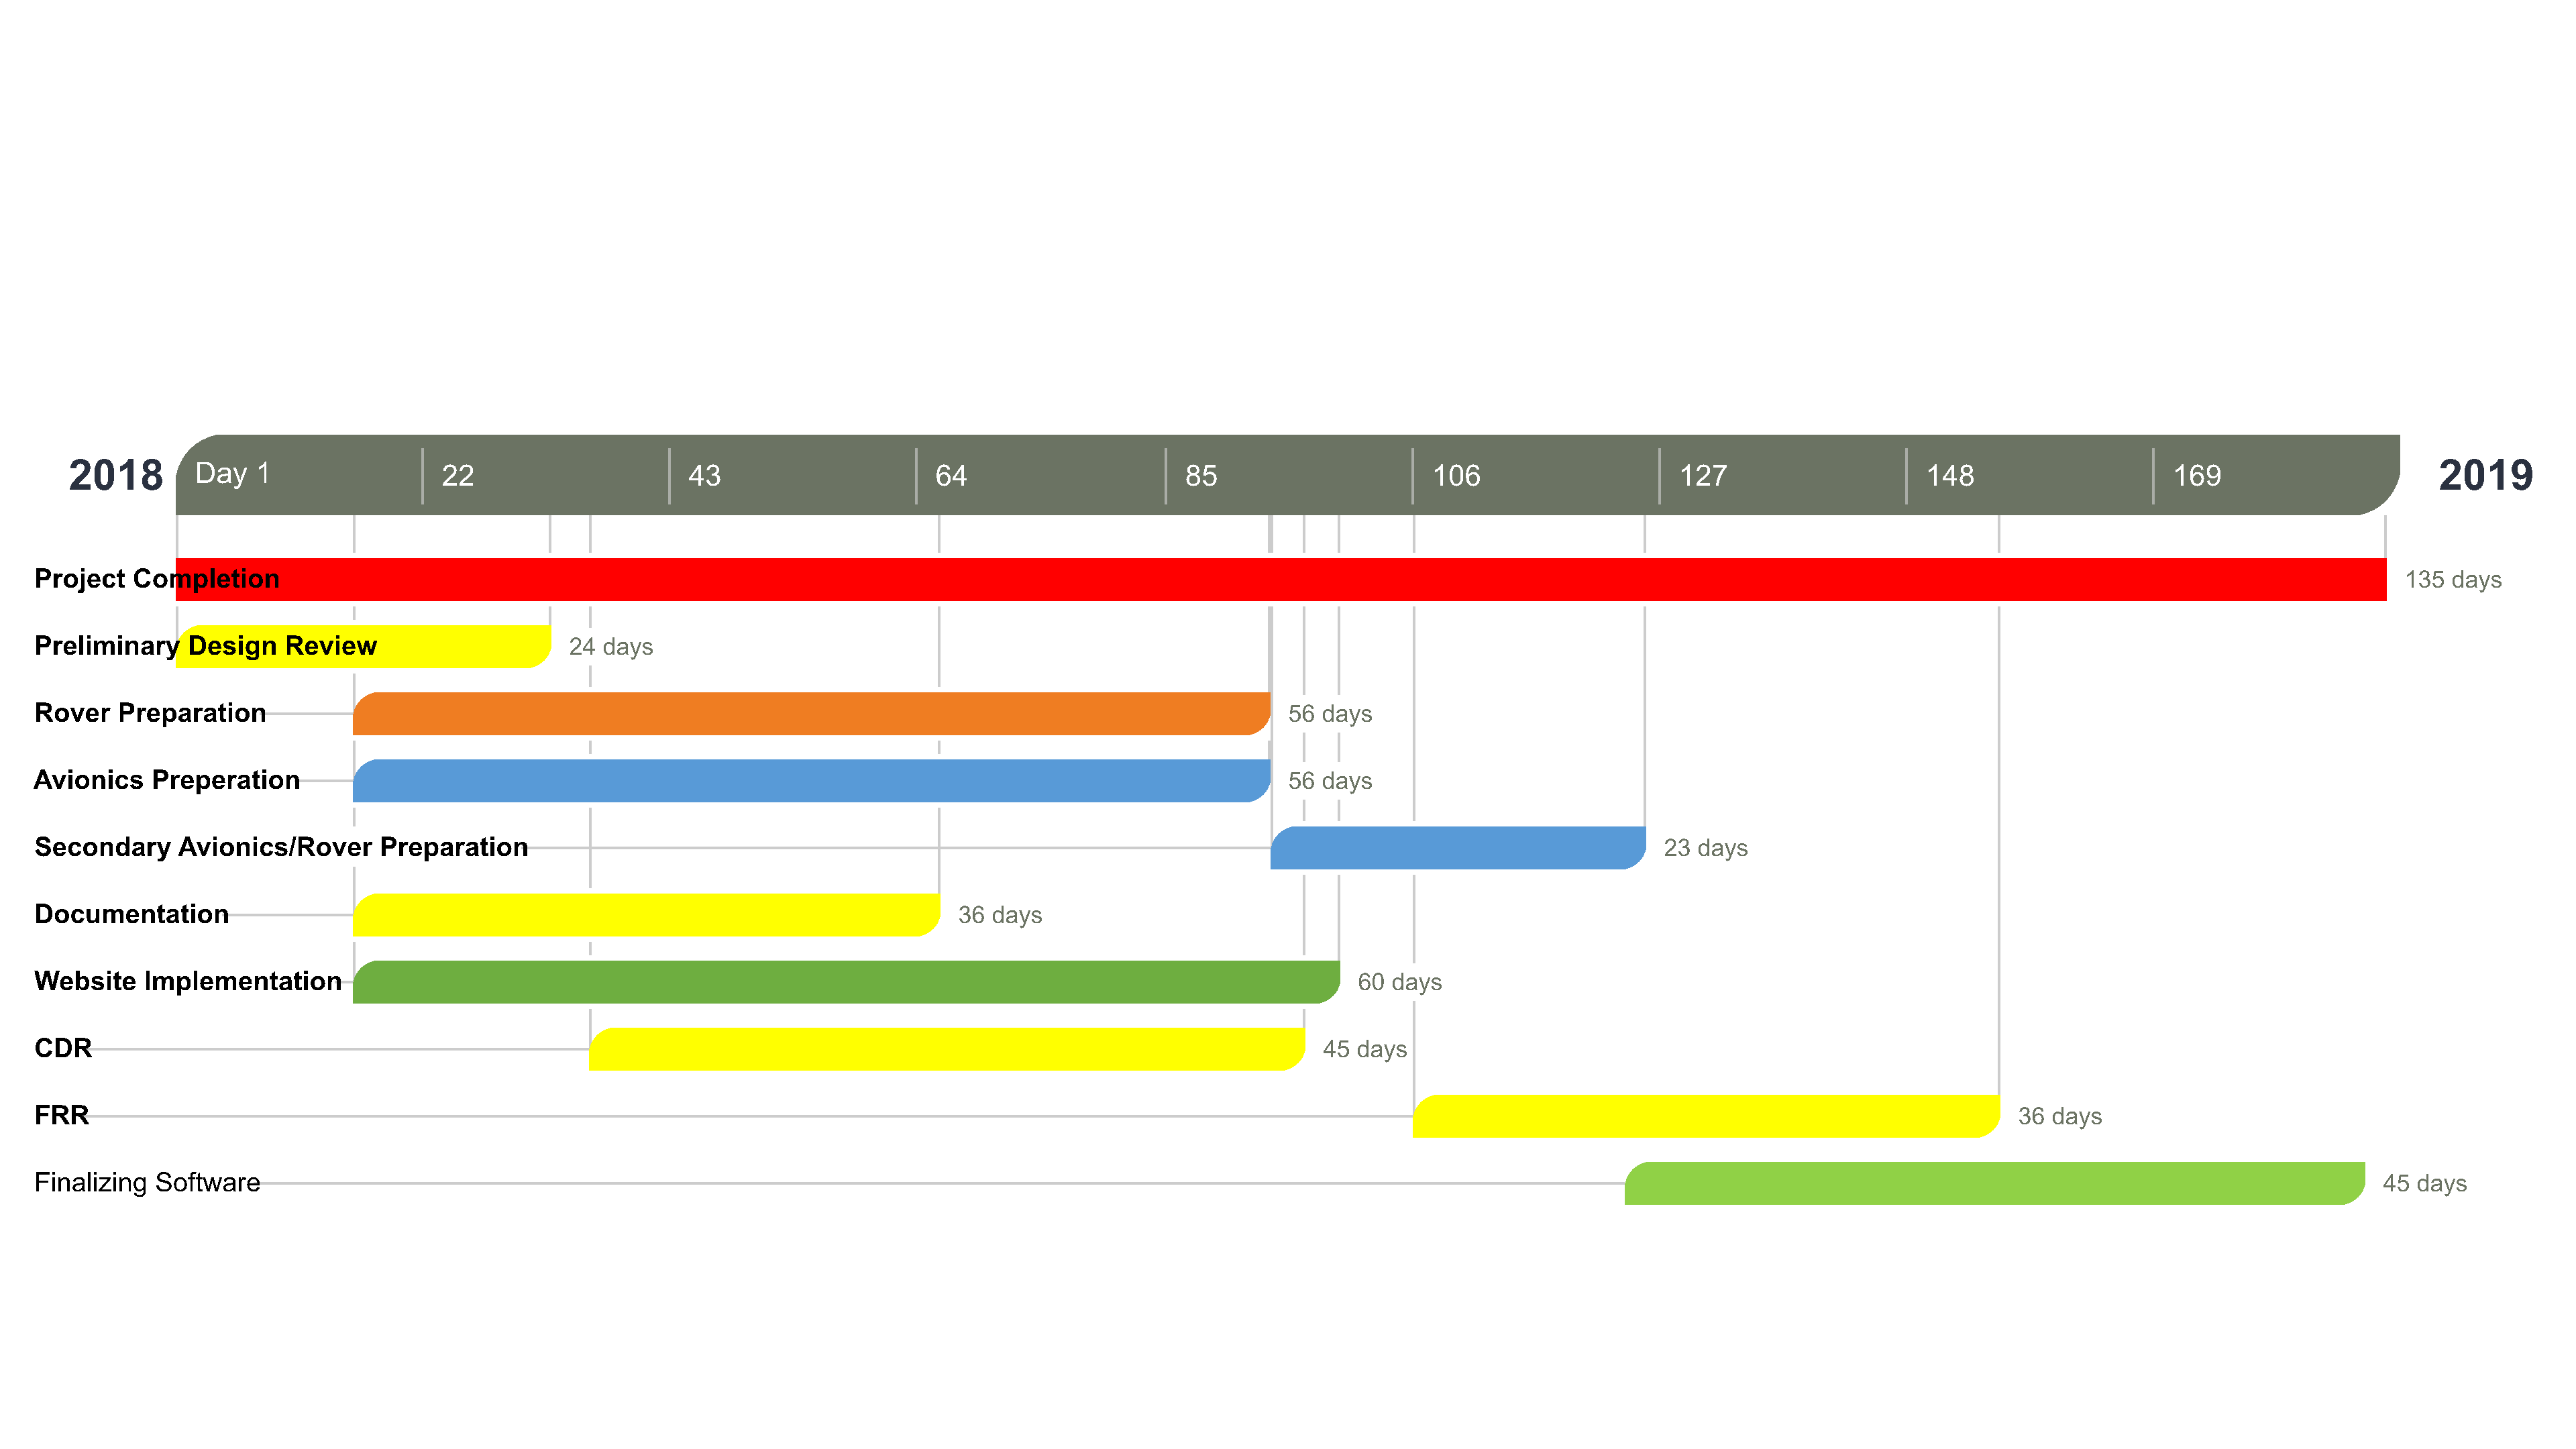
\includegraphics[width=\paperwidth]{PlanningRoadmap.png}} 
\end{center}


\end{document}